\documentclass[11pt]{article}
\usepackage[margin=1in]{geometry}
\usepackage{amsmath,amssymb,amsthm}
\usepackage{graphicx}
\usepackage[hidelinks]{hyperref}

\newtheorem{theorem}{Theorem}
\newtheorem{lemma}{Lemma}
\newtheorem{corollary}{Corollary}

\newcommand{\N}{\mathbb N}
\newcommand{\W}{\mathcal W}
\newcommand{\Lop}{\mathcal L}
\newcommand{\Kop}{\mathcal K}
\newcommand{\Wp}{\mathcal W_{(p,1)}}
\newcommand{\lpw}{\ell_p^w}
\newcommand{\linf}{\ell_\infty}
\newcommand{\ellone}{\ell_1}

\title{The weak $(p,1)$ limit case fails}
\author{Lane 19 packet for arXiv:1409.6476}
\date{2026-06-20}

\begin{document}
\maketitle

\section*{Source and target}

The source is Kati Ain and Eve Oja, \emph{On $(p,r)$-null sequences
and their relatives}, arXiv:1409.6476 \cite{ainoja}.  In Proposition
4.5 they prove, for $1\le p<\infty$ and $1<r\le p^\ast$ with
$r<\infty$ if $p=1$, that
\[
   \mathcal W_{(p,r)}=\mathcal W_{(p,r)}\circ\mathcal W
   \quad\text{and}\quad
   \mathbf w_{(p,r)}=\mathcal W_{(p,r)}(\mathbf w).
\]
Remark 4.6 asks whether this remains true in the limit case $r=1$.

\begin{center}
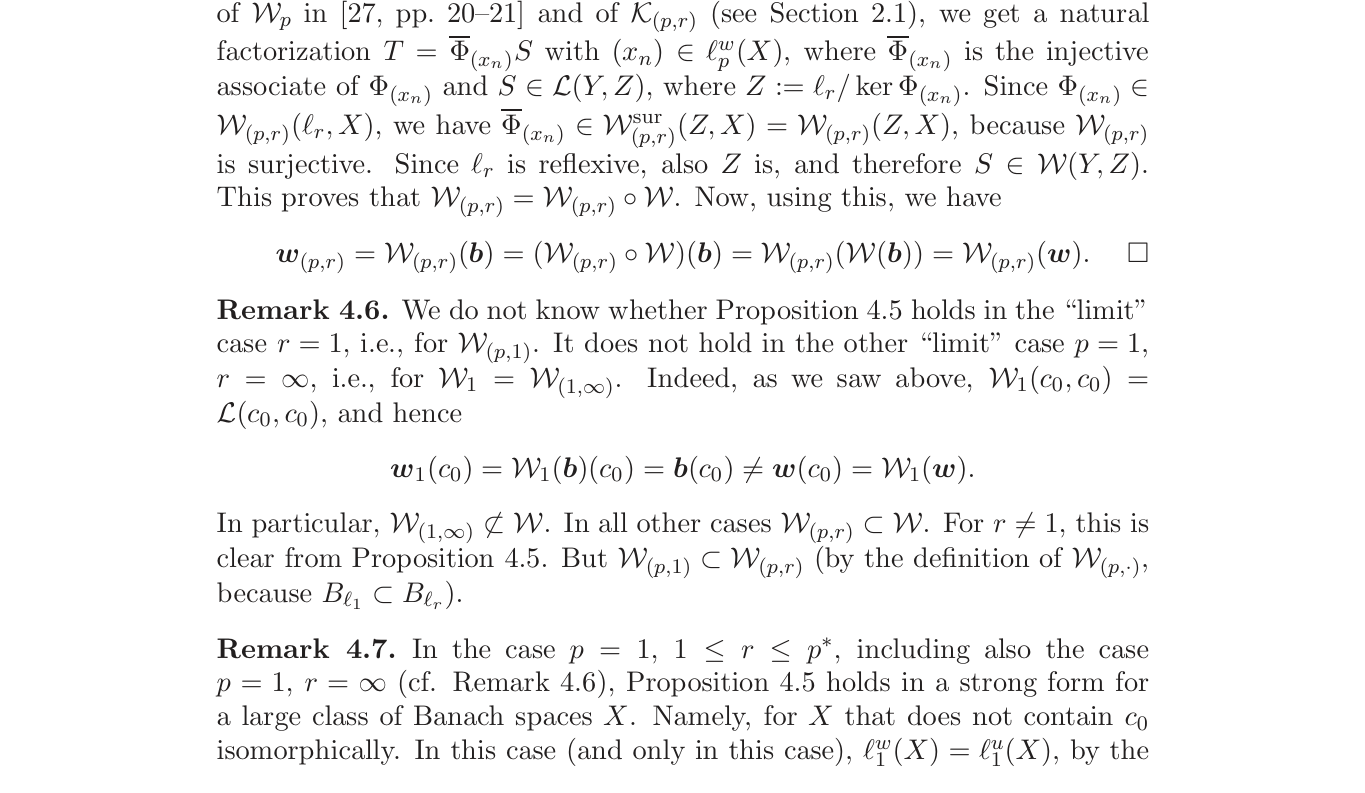
\includegraphics[width=\textwidth]{figures/prop45_limit_crop.png}
\end{center}

Theorem 4.8 gives an omnibus characterization of weakly $(p,r)$-null
sequences under the same non-limit hypotheses.  Remark 4.9 asks
whether Theorem 4.8 holds in the limit cases, including $r=1$.

\begin{center}
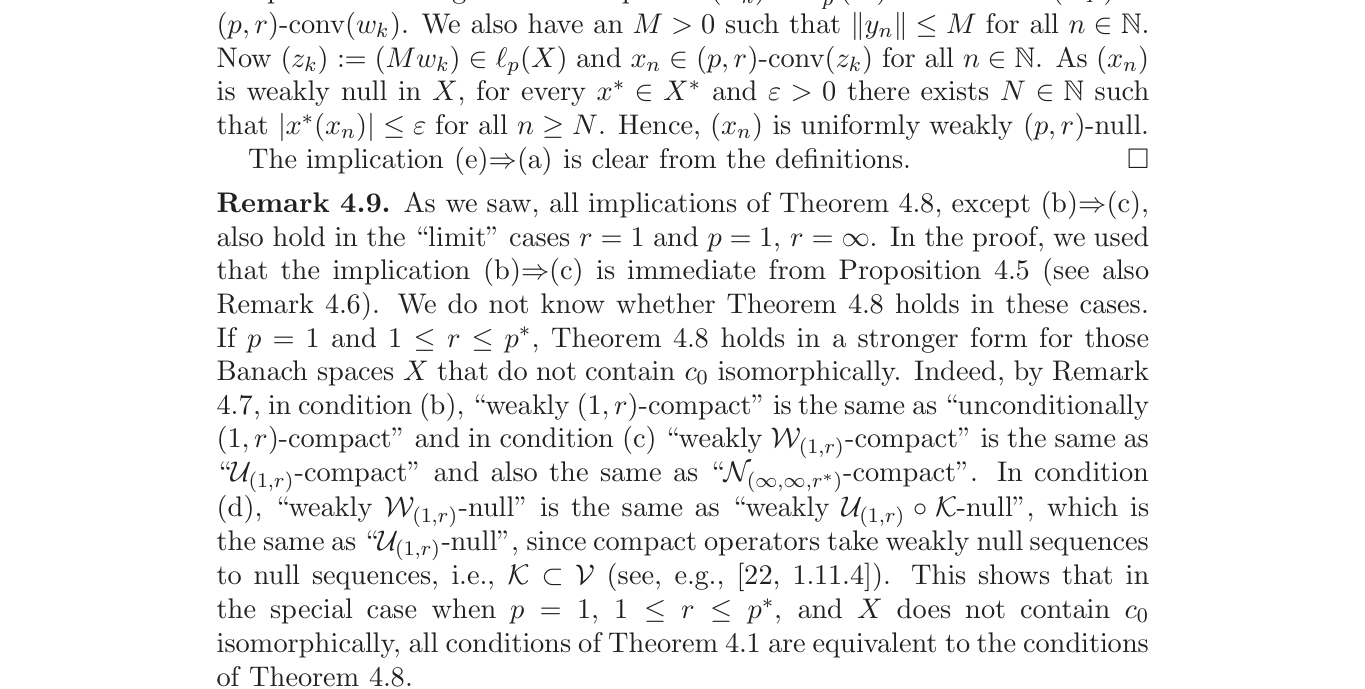
\includegraphics[width=\textwidth]{figures/thm48_limit_crop.png}
\end{center}

This packet gives a negative answer for $r=1$, for every
$1\le p<\infty$.

\section*{Definitions used}

For a sequence $(z_k)\in \ell_p^w(X)$, the weak $(p,1)$-convex hull is
\[
   (p,1)\operatorname{-conv}(z_k)
   =\left\{\sum_{k=1}^\infty a_k z_k:\ (a_k)\in B_{\ell_1}\right\}.
\]
An operator $T:Y\to X$ is weakly $(p,1)$-compact if
$T(B_Y)$ is contained in such a hull for some $(z_k)\in\ell_p^w(X)$.

\section*{Proof intuition}

The endpoint $r=1$ is special because the natural coefficient space is
$\ell_1$, whose quotients have the Schur property.  Thus every weakly
$(p,1)$-compact operator is completely continuous: after the standard
factorization through a quotient of $\ell_1$, weakly null sequences
become norm-null.  Therefore an operator in
$\mathcal W_{(p,1)}\circ\mathcal W$ maps bounded sets first to weakly
compact sets and then, by complete continuity, to norm-compact sets.
So every operator in the product ideal is compact.  But the canonical
inclusion $\ell_1\hookrightarrow c_0$ is weakly $(p,1)$-compact and
not compact.

\begin{lemma}\label{lem:cc}
For every $1\le p<\infty$, every weakly $(p,1)$-compact operator is
completely continuous.
\end{lemma}

\begin{proof}
Let $T:Y\to X$ be weakly $(p,1)$-compact.  Then there is
$(z_k)\in\ell_p^w(X)$ such that
\[
   T(B_Y)\subseteq \Phi(B_{\ell_1}),
   \qquad
   \Phi(a)=\sum_{k=1}^\infty a_kz_k .
\]
The map $\Phi:\ell_1\to X$ is bounded because $(z_k)$ is weakly
$p$-summable and hence bounded.  Let $q:\ell_1\to Z=\ell_1/\ker\Phi$
be the quotient map and let $\overline\Phi:Z\to X$ be the induced
injective operator.  Since $T(B_Y)\subseteq \Phi(B_{\ell_1})$,
$T$ takes values in $\operatorname{ran}\Phi$, and the formula
\[
   Sy=q(a)\quad\text{whenever }\Phi a=Ty
\]
defines a bounded linear map $S:Y\to Z$ with $T=\overline\Phi S$.
Indeed, for $\|y\|\le1$ one may choose $a\in B_{\ell_1}$ with
$\Phi a=Ty$, so $\|Sy\|\le1$ in the quotient norm.

The space $Z$ has the Schur property, because it is a quotient of
$\ell_1$.  If $y_n\to0$ weakly in $Y$, then $Sy_n\to0$ weakly in $Z$,
hence $\|Sy_n\|\to0$.  Therefore
\[
   \|Ty_n\|=\|\overline\Phi Sy_n\|\to0.
\]
So $T$ is completely continuous.
\end{proof}

\begin{lemma}\label{lem:productcompact}
For every $1\le p<\infty$,
\[
   \mathcal W_{(p,1)}\circ\mathcal W \subseteq \mathcal K .
\]
\end{lemma}

\begin{proof}
Let $T=A B$ where $B:Y\to Z$ is weakly compact and
$A:Z\to X$ is weakly $(p,1)$-compact.  By Lemma \ref{lem:cc}, $A$ is
completely continuous.

The set $B(B_Y)$ is relatively weakly compact.  By Eberlein--Smulian,
every sequence in $B(B_Y)$ has a weakly convergent subsequence.  If
$z_{n_j}\to z$ weakly in $Z$, then $z_{n_j}-z\to0$ weakly, hence
$A z_{n_j}\to A z$ in norm by complete continuity.  Thus
$A(B(B_Y))=T(B_Y)$ is relatively norm sequentially compact, hence
relatively norm compact.  Therefore $T$ is compact.
\end{proof}

\begin{theorem}\label{thm:prop45fails}
For every $1\le p<\infty$,
\[
   \mathcal W_{(p,1)}\ne \mathcal W_{(p,1)}\circ\mathcal W .
\]
\end{theorem}

\begin{proof}
Let $j:\ell_1\to c_0$ be the canonical inclusion.  We first show that
$j\in\mathcal W_{(p,1)}$.

Let $(e_k)$ be the unit vector basis of $c_0$.  Since $(c_0)^\ast=\ell_1$
and $\ell_1\subseteq \ell_p$ for $1\le p<\infty$, the sequence
$(e_k)$ belongs to $\ell_p^w(c_0)$.  Moreover,
\[
   j(B_{\ell_1})
   =
   \left\{\sum_{k=1}^\infty a_ke_k:\ (a_k)\in B_{\ell_1}\right\}
   =
   (p,1)\operatorname{-conv}(e_k).
\]
Thus $j$ is weakly $(p,1)$-compact.

But $j$ is not compact, since $(j e_k)=(e_k)$ has no norm-convergent
subsequence in $c_0$.  Lemma \ref{lem:productcompact} says that every
operator in $\mathcal W_{(p,1)}\circ\mathcal W$ is compact.  Hence
$j\notin \mathcal W_{(p,1)}\circ\mathcal W$, proving the strict
inequality.
\end{proof}

\begin{corollary}\label{cor:thm48fails}
Theorem 4.8 of the source does not extend to the limit case $r=1$.
More precisely, for every $1\le p<\infty$, condition (b) of Theorem
4.8 does not imply condition (c) when $r=1$.
\end{corollary}

\begin{proof}
In $X=c_0$, take $x_n=e_n$.  The sequence $(e_n)$ is weakly null in
$c_0$, because every functional on $c_0$ is an $\ell_1$ sequence.
As above, $(e_k)\in\ell_p^w(c_0)$ and
$e_n\in (p,1)\operatorname{-conv}(e_k)$ for every $n$.  Thus
$(e_n)$ is weakly null and relatively weakly $(p,1)$-compact, which is
condition (b) of Theorem 4.8 with $r=1$.

Suppose condition (c) held.  Then $\{e_n:n\in\N\}$ would be weakly
$\mathcal W_{(p,1)}$-compact: there would be a weakly $(p,1)$-compact
operator $A:Y\to c_0$ and a relatively weakly compact set
$K\subseteq Y$ with
\[
   \{e_n:n\in\N\}\subseteq A(K).
\]
By Lemma \ref{lem:cc}, $A$ is completely continuous, so the same
Eberlein--Smulian argument as in Lemma \ref{lem:productcompact} shows
that $A(K)$ is norm compact.  This is impossible because the set
$\{e_n:n\in\N\}$ has no norm-convergent subsequence in $c_0$.
\end{proof}

\section*{Verification and limitations}

The counterexample is in ZFC and works for every $1\le p<\infty$.
It answers the source's $r=1$ limit question negatively.  It does not
address any positive endpoint behavior under extra hypotheses, such as
the source's no-$c_0$ hypothesis in Remark 4.9.

Bounded novelty checks were performed on 2026-06-20 against the local
run indexes, the local parsed arXiv corpus, and web searches for exact
and close phrases around Proposition 4.5, Theorem 4.8, $r=1$, and
weakly $(p,1)$-compact operators.  These checks found the source paper
and no prior answer to the endpoint question.

\begin{thebibliography}{9}

\bibitem{ainoja}
K. Ain and E. Oja,
\emph{On $(p,r)$-null sequences and their relatives},
arXiv:1409.6476, 2014.

\bibitem{megginson}
R. E. Megginson,
\emph{An Introduction to Banach Space Theory},
Graduate Texts in Mathematics 183, Springer, 1998.

\end{thebibliography}

\end{document}

